\documentclass[floatsintext,man]{apa6}

\usepackage{amssymb,amsmath}
\usepackage{ifxetex,ifluatex}
\usepackage{fixltx2e} % provides \textsubscript
\ifnum 0\ifxetex 1\fi\ifluatex 1\fi=0 % if pdftex
  \usepackage[T1]{fontenc}
  \usepackage[utf8]{inputenc}
\else % if luatex or xelatex
  \ifxetex
    \usepackage{mathspec}
    \usepackage{xltxtra,xunicode}
  \else
    \usepackage{fontspec}
  \fi
  \defaultfontfeatures{Mapping=tex-text,Scale=MatchLowercase}
  \newcommand{\euro}{€}
\fi
% use upquote if available, for straight quotes in verbatim environments
\IfFileExists{upquote.sty}{\usepackage{upquote}}{}
% use microtype if available
\IfFileExists{microtype.sty}{\usepackage{microtype}}{}

% Table formatting
\usepackage{longtable, booktabs}
\usepackage{lscape}
% \usepackage[counterclockwise]{rotating}   % Landscape page setup for large tables
\usepackage{multirow}		% Table styling
\usepackage{tabularx}		% Control Column width
\usepackage[flushleft]{threeparttable}	% Allows for three part tables with a specified notes section
\usepackage{threeparttablex}            % Lets threeparttable work with longtable

% Create new environments so endfloat can handle them
% \newenvironment{ltable}
%   {\begin{landscape}\begin{center}\begin{threeparttable}}
%   {\end{threeparttable}\end{center}\end{landscape}}

\newenvironment{lltable}
  {\begin{landscape}\begin{center}\begin{ThreePartTable}}
  {\end{ThreePartTable}\end{center}\end{landscape}}




% The following enables adjusting longtable caption width to table width
% Solution found at http://golatex.de/longtable-mit-caption-so-breit-wie-die-tabelle-t15767.html
\makeatletter
\newcommand\LastLTentrywidth{1em}
\newlength\longtablewidth
\setlength{\longtablewidth}{1in}
\newcommand\getlongtablewidth{%
 \begingroup
  \ifcsname LT@\roman{LT@tables}\endcsname
  \global\longtablewidth=0pt
  \renewcommand\LT@entry[2]{\global\advance\longtablewidth by ##2\relax\gdef\LastLTentrywidth{##2}}%
  \@nameuse{LT@\roman{LT@tables}}%
  \fi
\endgroup}


  \usepackage{graphicx}
  \makeatletter
  \def\maxwidth{\ifdim\Gin@nat@width>\linewidth\linewidth\else\Gin@nat@width\fi}
  \def\maxheight{\ifdim\Gin@nat@height>\textheight\textheight\else\Gin@nat@height\fi}
  \makeatother
  % Scale images if necessary, so that they will not overflow the page
  % margins by default, and it is still possible to overwrite the defaults
  % using explicit options in \includegraphics[width, height, ...]{}
  \setkeys{Gin}{width=\maxwidth,height=\maxheight,keepaspectratio}
\ifxetex
  \usepackage[setpagesize=false, % page size defined by xetex
              unicode=false, % unicode breaks when used with xetex
              xetex]{hyperref}
\else
  \usepackage[unicode=true]{hyperref}
\fi
\hypersetup{breaklinks=true,
            pdfauthor={},
            pdftitle={Equivalence Testing and the Second Generation P-Value},
            colorlinks=true,
            citecolor=blue,
            urlcolor=blue,
            linkcolor=black,
            pdfborder={0 0 0}}
\urlstyle{same}  % don't use monospace font for urls

\setlength{\parindent}{0pt}
%\setlength{\parskip}{0pt plus 0pt minus 0pt}

\setlength{\emergencystretch}{3em}  % prevent overfull lines


% Manuscript styling
\captionsetup{font=singlespacing,justification=justified}
\usepackage{csquotes}
\usepackage{upgreek}



\usepackage{tikz} % Variable definition to generate author note

% fix for \tightlist problem in pandoc 1.14
\providecommand{\tightlist}{%
  \setlength{\itemsep}{0pt}\setlength{\parskip}{0pt}}

% Essential manuscript parts
  \title{Equivalence Testing and the Second Generation \emph{P}-Value}

  \shorttitle{TOST vs.~SGPV}


  \author{Daniël Lakens\textsuperscript{1}~\& Marie Delacre\textsuperscript{2}}

  \def\affdep{{"", ""}}%
  \def\affcity{{"", ""}}%

  \affiliation{
    \vspace{0.5cm}
          \textsuperscript{1} Eindhoven University of Technology, Eindhoven, The Netherlands\\
          \textsuperscript{2} Service of Analysis of the Data, Université Libre de Bruxelles, Belgium  }

  \authornote{
    \newcounter{author}
    All code associated with this article, including the reproducible
    manuscript, is available from
    \url{https://github.com/Lakens/TOST_vs_SGPV}. This work was supported by
    the Netherlands Organization for Scientific Research (NWO) VIDI grant
    452-17-013.

                      Correspondence concerning this article should be addressed to Daniël Lakens, Den Dolech 1, IPO 1.33, 5600 MB, Eindhoven, The Netherlands. E-mail: \href{mailto:D.Lakens@tue.nl}{\nolinkurl{D.Lakens@tue.nl}}
                          }


  \abstract{To move beyond the limitations of null-hypothesis tests, statistical
approaches have been developed where the observed data is compared
against a range of values that are equivalent to the absence of a
meaningful effect. Specifying a range of values around zero allows
researchers to statistically reject the presence of effects large enough
to matter, and prevents practically insignificant effects from being
interpreted as a statistically significant difference. We compare the
behavior of the recently proposed second generation \emph{p}-value
(Blume, D'Agostino McGowan, Dupont, \& Greevy, 2018) with the more
established Two One-Sided Tests (TOST) equivalence testing procedure
(Schuirmann, 1987). We show that the two approaches yield almost
identical results under optimal conditions. Under suboptimal conditions
(e.g., when the confidence interval is wider than the equivalence range,
or when confidence intervals are asymmetric) the second generation
\emph{p}-value becomes difficult to interpret as a descriptive
statistic. The second generation \emph{p}-value is interpretable in a
dichotomous manner (i.e., when the SGPV equals 0 or 1 because the
confidence intervals lies completely within or outside of the
equivalence range), but this dichotomous interpretation does not require
calculations. We conclude that equivalence tests yield more consistent
\emph{p}-values, distinguish between datasets that yield the same second
generation \emph{p}-value, and allow for easier control of Type I and
Type II error rates.}
  \keywords{equivalence testing, second generation \emph{p}-values, hypothesis
testing, TOST, statistical inference \\

    
  }





\usepackage{amsthm}
\newtheorem{theorem}{Theorem}
\newtheorem{lemma}{Lemma}
\theoremstyle{definition}
\newtheorem{definition}{Definition}
\newtheorem{corollary}{Corollary}
\newtheorem{proposition}{Proposition}
\theoremstyle{definition}
\newtheorem{example}{Example}
\theoremstyle{definition}
\newtheorem{exercise}{Exercise}
\theoremstyle{remark}
\newtheorem*{remark}{Remark}
\newtheorem*{solution}{Solution}
\begin{document}

\maketitle

\setcounter{secnumdepth}{0}



To test predictions researchers predominantly rely on null-hypothesis
tests.\\
This statistical approach can be used to examine whether observed data
is sufficiently surprising under the null hypothesis to reject an effect
that equals exactly zero. Null-hypothesis tests have an important
limitation, in that this procedure can only reject the hypothesis that
there is no effect, while scientists should also be able to provide
statistical support for \emph{equivalence}. When testing for equivalence
researchers aim to examine whether an observed effect is too small to be
considered meaningful, and therefore is practically equivalent to zero.
By specifying a range around the null hypothesis of values that are
deemed practically equivalent to the absence of an effect (i.e., 0 ±
0.3) the observed data can be compared against an \emph{equivalence
range} and researchers can test if a meaningful effect is absent (Hauck
\& Anderson, 1984; Kruschke, 2018; Rogers, Howard, \& Vessey, 1993;
Serlin \& Lapsley, 1985; Spiegelhalter, Freedman, \& Parmar, 1994;
Wellek, 2010; Westlake, 1972).

Second generation \emph{p}-values (SGPV) were recently proposed to as a
descriptive statistic that represents \enquote{the proportion of
data-supported hypotheses that are also null hypotheses} (Blume et al.,
2018). The researcher specifies an equivalence range around a null
hypothesis of values that are considered practically equivalent to the
null hypothesis. The SGPV measures the degree to which a set of
data-supported parameter values falls within the interval null
hypothesis. If the estimation interval falls completely within the
equivalence range, the SGPV is 1. If the confidence interval falls
completely outside of the equivalence range, the SGPV is 0. Otherwise
the SGPV is a value between 0 and 1 that expresses the overlap of
data-supported hypotheses and the equivalence range. When calculating
the SGPV the set of data-supported parameter values can be represented
by a confidence interval (CI), although one could also choose to use
credible intervals or Likelihood support intervals (SI). When a
confidence interval is used, the SGPV and equivalence tests such as the
Two One-Sided Tests (TOST) procedure (Lakens, 2017; Meyners, 2012;
Quertemont, 2011; Schuirmann, 1987) appear to have close ties, because
both tests compare a confidence interval against an equivalence range.
Here, we aim to examine the similarities and differences between the
TOST procedure and the SGPV.

The TOST procedure also relies on the confidence interval around the
effect. In the TOST procedure the data is tested against the lower
equivalence bound in the first one-sided test, and against the upper
equivalence bound in the second one-sided test (Lakens, Scheel, \&
Isager, 2018). If both tests statistically reject an effect as extreme
or more extreme than the equivalence bound, you can conclude the
observed effect is practically equivalent to zero from a Neyman-Pearson
approach to statistical inferences. Because one-sided tests are
performed, one can also conclude equivalence by checking whether the
1-2\(\times\)\(\alpha\) confidence interval (e.g., when the alpha level
is 0.05, a 90\% CI) falls completely within the equivalence bounds.
Because both equivalence tests as the SGPV are based on whether and how
much a confidence interval overlaps with equivalence bounds, it seems
worthwhile to compare the behavior of the newly proposed SGPV to
equivalence tests to examine the unique contribution of the SGPV to the
statistical toolbox.

\section{\texorpdfstring{The relationship between \emph{p}-values from
TOST and SGPV when confidence intervals are
symmetrical}{The relationship between p-values from TOST and SGPV when confidence intervals are symmetrical}}\label{the-relationship-between-p-values-from-tost-and-sgpv-when-confidence-intervals-are-symmetrical}

The second generation \emph{p}-value (SGPV) is calculated as: \[
  p _ { \delta } = \frac { \left| I \cap H _ { 0 } \right| } { | I | } \times \max \left\{ \frac { | I | } { 2 \left| H _ { 0 } \right| } , 1 \right\}
\] where I is the interval based on the data (e.g., a 95\% confidence
interval) and H\textsubscript{0} is the equivalence range. The first
term of this formula implies that the second generation \emph{p}-value
is the width of the confidence interval that overlaps with the
equivalence range, divided by the total width of the confidence
interval. The second term is a \enquote{small sample correction} (which
will be discussed later) that comes into play whenever the confidence
interval is more than twice as wide as the equivalence range. To examine
the relation between the TOST \emph{p}-value and the SGPV we can
calculate both statistics across a range of observed effect sizes. In
Figure \ref{fig:TOSTSGPV1} \emph{p}-values are plotted for the TOST
procedure and the SGPV. The statistics are calculated for hypothetical
one-sample \emph{t}-tests for observed means ranging from 140 to 150 (on
the x-axis). The equivalence range is set to 145 ± 2 (i.e., an
equivalence range from 143 to 147), the observed standard deviation is
assumed to be 2, and the sample size is 30. For example, for the
left-most point in Figure \ref{fig:TOSTSGPV1} the SGPV and the TOST
\emph{p}-value is calculated for a hypothetical study with a sample size
of 30, an observed standard deviation of 2, and an observed mean of 140,
where the \emph{p}-value for the equivalence test is 1, and the SGPV is
0. Our conclusions about the relationship between TOST \emph{p}-values
and SGPV in this article are not dependent upon any specific example, as
readers can explore for themselves in an online Shiny app:
\url{http://shiny.ieis.tue.nl/TOST_vs_SGPV/}.

\begin{figure}
\centering
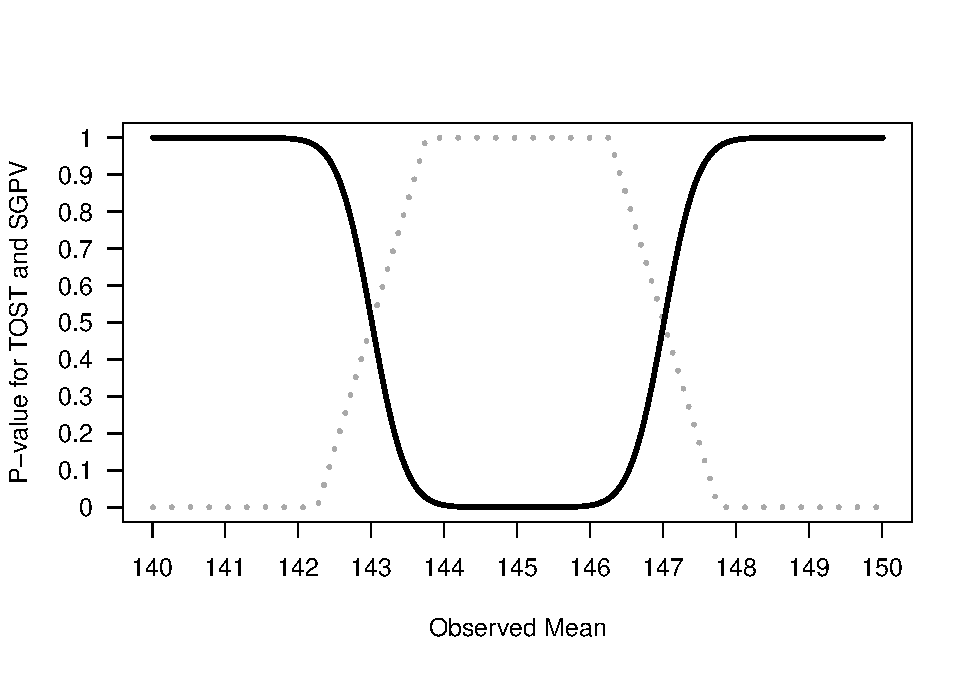
\includegraphics{manuscript_files/figure-latex/TOSTSGPV1-1.pdf}
\caption{\label{fig:TOSTSGPV1}Comparison of \emph{p}-values from TOST (black
line) and SGPV (dotted grey line) across a range of observed sample
means (x-axis) tested against a mean of 145 in a one-sample
\emph{t}-test with a sample size of 30 and a standard deviation of 2.}
\end{figure}

The SGPV treats the equivalence range as the null-hypothesis, while the
TOST procedure treats the values outside of the equivalence range as the
null-hypothesis. For ease of comparison we can reverse the SGPV (by
calculating 1-SGPV in Figure \ref{fig:TOSTSGPV2}) to make the values
more easily comparable. We see that the \emph{p}-value from the TOST
procedure and the SGPV follow each other closely.

\begin{figure}
\centering
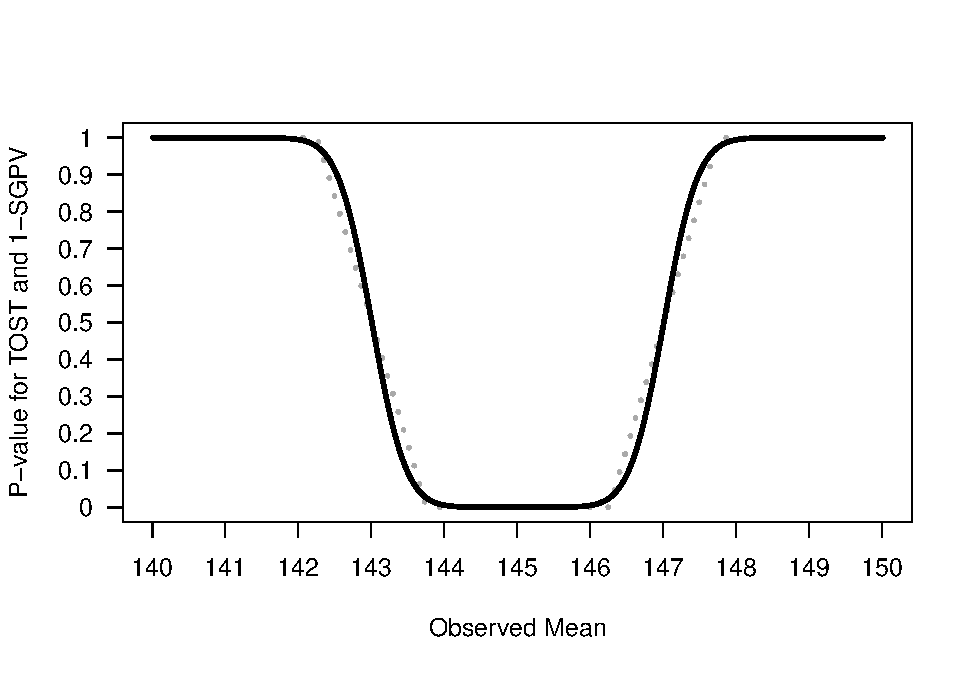
\includegraphics{manuscript_files/figure-latex/TOSTSGPV2-1.pdf}
\caption{\label{fig:TOSTSGPV2}Comparison of \emph{p}-values from TOST (black
line) and 1-SGPV (dotted grey line) across a range of observed sample
means (x-axis) tested against a mean of 145 in a one-sample
\emph{t}-test with a sample size of 30 and a standard deviation of 2.}
\end{figure}

When the observed sample mean is 145, the sample size is 30, and the
standard deviation is 2, and we are testing against equivalence bounds
of 143 and 147 using the TOST procedure for a one-sample \emph{t}-test,
the equivalence test is significant, \emph{t}(29) = 5.48, \emph{p}
\textless{} .001. Because the 95\% CI falls completely within the
equivalence bounds, the SGPV is 1 (see Figure \ref{fig:TOSTSGPV1}). On
the other hand, when the observed mean is 140, the equivalence test is
not significant (the observed mean is far outside the equivalence range
of 143 to 147), \emph{t}(29) = -8.22, \emph{p} = 1 (or more accurately,
\emph{p} \textgreater{} .999 as \emph{p}-values are bounded between 0
and 1). Because the 95\% CI falls completely outside the equivalence
bounds, the SGPV is 0 (see Figure \ref{fig:TOSTSGPV1}).

\subsection{SGPV as a uniform measure of
overlap}\label{sgpv-as-a-uniform-measure-of-overlap}

It is clear the SGPV and the \emph{p}-value from TOST are closely
related. When confidence intervals are symmetric we can think of the
SGPV as a straight line that is directly related to the \emph{p}-value
from an equivalence test for three values. When the TOST \emph{p}-value
is 0.5, the SGPV is also 0.5 (note that the reverse is not true). The
SGPV is 50\% when the observed mean falls exactly on the lower or upper
equivalence bound, because 50\% of the symmetrical confidence interval
overlaps with the equivalence range. When the observed mean equals the
equivalence bound, the difference between the mean in the data and the
equivalence bound is 0, the \emph{t}-value for the equivalence test is
also 0, and thus the \emph{p}-value is 0.5 (situation A, Figure
\ref{fig:TOSTSGPV3}).

\begin{figure}
\centering
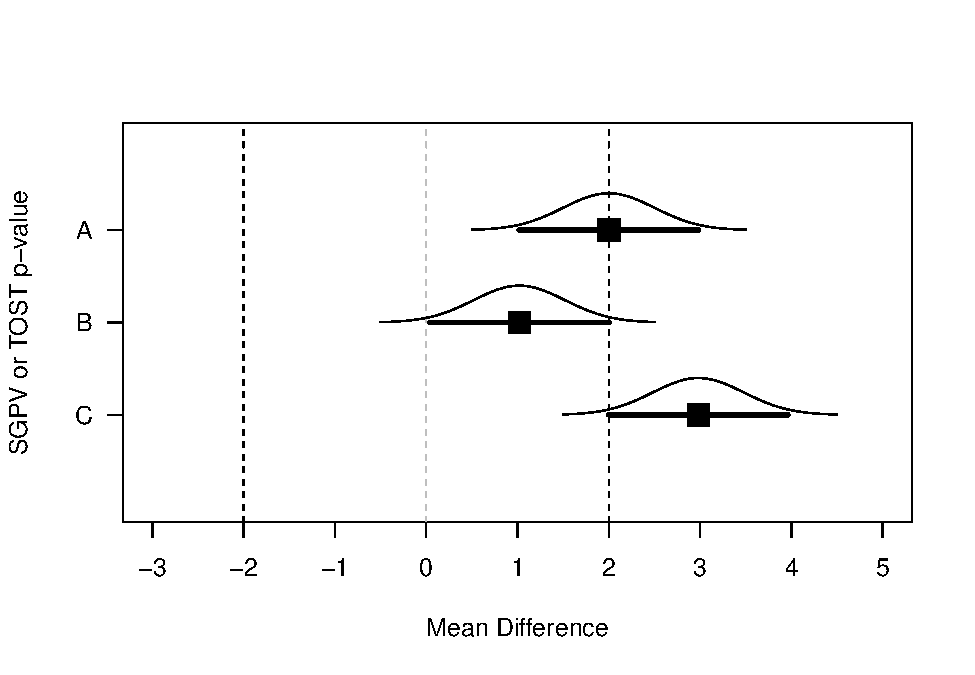
\includegraphics{manuscript_files/figure-latex/TOSTSGPV3-1.pdf}
\caption{\label{fig:TOSTSGPV3}Means, normal distribution, and 95\% CI for
three example datasets that illustrate the relationship between
\emph{p}-values from TOST and SGPV.}
\end{figure}

Two other points always have to overlap. When the 95\% CI falls
completely inside the equivalence region, and one endpoint of the
confidence interval is exactly equal to one of the equivalence bounds
(see situation B in Figure \ref{fig:TOSTSGPV3}) the TOST \emph{p}-value
(which relies on a one-sided test) is always 0.025. The third point
where the SGPV and the \emph{p}-value from the TOST procedure should
overlap is where the 95\% CI falls completely outside of the equivalence
range, but one endpoint of the confidence interval is equal to the
equivalence bound (see situation C in Figure \ref{fig:TOSTSGPV3}), when
the \emph{p}-value will always be 0.975. Note that this situation is in
essence a minimum-effect test (Murphy, Myors, \& Wolach, 2014). The goal
of a minimum-effect is not just to reject a difference of zero, but to
reject the smallest effect size of interest (i.e., the equivalence
bounds). The SGPV summarizes the information from an equivalence test
and a minimum-effect test. These can be two relevant questions to ask,
although it often makes sense to combine an equivalence test and a
null-hypothesis test instead (Lakens et al., 2018).

\begin{figure}
\centering
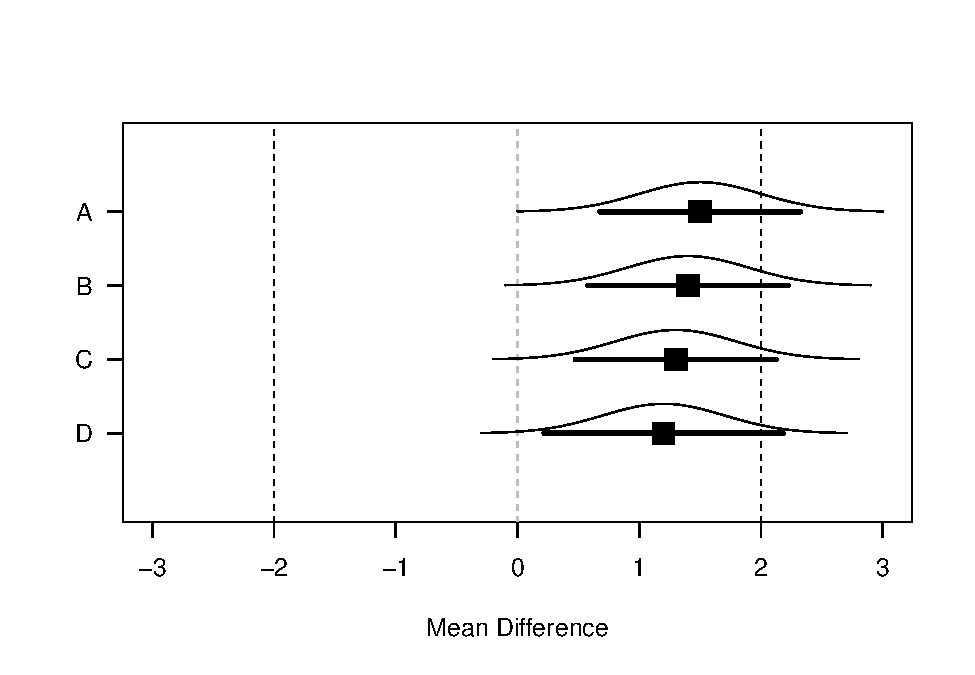
\includegraphics{manuscript_files/figure-latex/TOSTSGPV4-1.pdf}
\caption{\label{fig:TOSTSGPV4}Means, normal distribution, and 95\% CI for
samples where the observed population mean is 1.5, 1.4, 1.3, and 1.2.}
\end{figure}

For example, the SGPV from A to D is 0.76, 0.81, 0.86, and 0.91. The
difference in the percentage of overlap between A and B (-0.05) is
identical to the difference in the percentage of overlap between C and D
as the mean gets 0.1 closer to the test value (-0.05). As the observed
mean in a one-sample \emph{t}-test lies closer to the test value (in
Figure \ref{fig:TOSTSGPV4}), from situation A to D, the mean gets closer
to the test value by 0.1) the difference in the overlap changes
uniformly. As we move the observed mean closer to the test value in
steps of 0.1 across A to D the \emph{p}-value calculated for normally
distributed data is not uniformly distributed. The probability of
observing data more extreme than the upper bound of 2 is (from A to D)
0.16, 0.12, 0.08, and 0.06. As we can see, the difference between A and
B (0.04) is not the same as the difference between C and D (0.03).
Indeed, the difference in \emph{p}-values is the largest as you start at
\emph{p} = 0.5 (when the observed mean falls on the test value), which
is why the line in Figure \ref{fig:TOSTSGPV1} is the steepest at
\emph{p} = 0.5. Note that where the SGPV reaches 1 or 0, \emph{p}-values
closely approximate 0 and 1, but never reach these values.

\subsection{When are the SGPV and Equivalence Test
Unrelated?}\label{when-are-the-sgpv-and-equivalence-test-unrelated}

There are three situations where \emph{p}-values from TOST and SGPV are
unrelated. The first two situations were discussed before and can be
seen in Figure \ref{fig:TOSTSGPV1}. When the SGPV is either 0 or 1
\emph{p}-values from the equivalence test fall between 0.975 and 1 or
between 0 and 0.025. Because \emph{p}-values approach 0 or 1, but are
never exactly 0 or 1, and the SGPV is exactly 0 or 1, the two statistics
are completely unrelated within these ranges. The easiest way to see
this is by plotting the SGPV against the \emph{p}-value from the TOST
procedure. The situations where the SPGV and \emph{p}-values from the
TOST procedure are unrelated are indicated by the parts of the curve
where there are vertical straight lines at second generation
\emph{p}-values of 0 and 1.

\begin{figure}
\centering
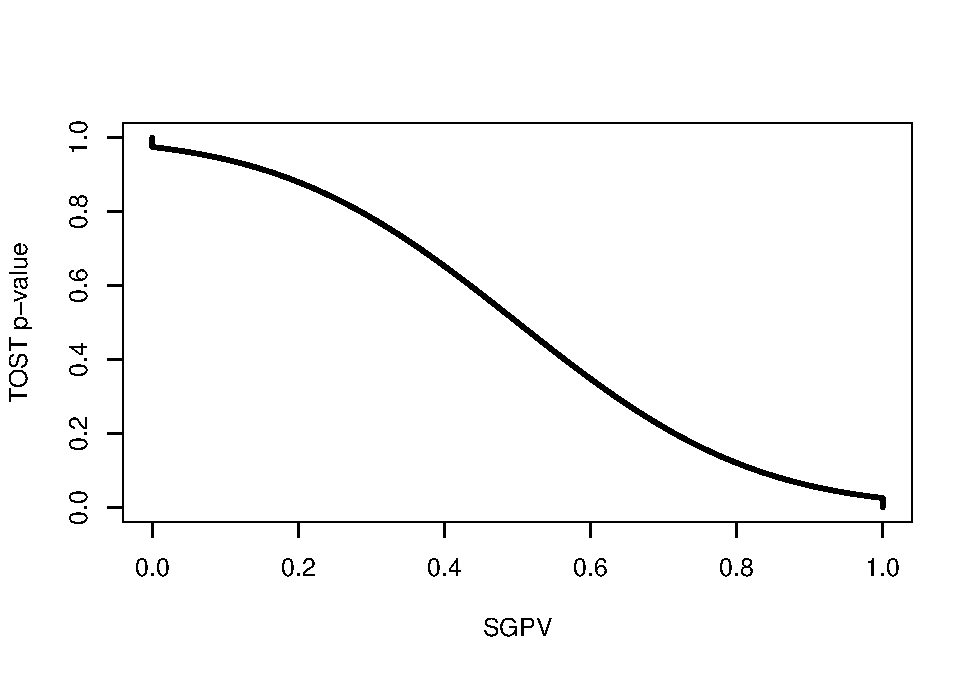
\includegraphics{manuscript_files/figure-latex/TOSTSGPV5-1.pdf}
\caption{\label{fig:TOSTSGPV5}The relationship between \emph{p}-values from
the TOST procedure and the SGPV for the same scenario as in Figure
\ref{fig:TOSTSGPV1}.}
\end{figure}

A third situation in which the SGPV deviates from the TOST
\emph{p}-value is whenever the CI is wider than the equivalence range,
and the CI overlaps with the upper \emph{and} lower equivalence bound.
When the confidence interval is more than twice as wide as the
equivalence range the SGPV is set to 0.5. Blume et al. (2018) call this
the \enquote{small sample correction factor}. However, it is not a
correction in the typical sense of the word, since the SGPV is not
adjusted to any \enquote{correct} value. When the normal calculation
would be \enquote{misleading} (i.e., the SGPV would be small, which
normally would suggest support for the alternative hypothesis, but at
the same time all values in the equivalence range are supported), the
SGPV is set to 0.5 which according to Blume and colleagues signals that
the SGPV is \enquote{uninformative}. Note that the CI can be twice as
wide as the equivalence range whenever the sample size is small (and the
confidence interval width is large) \emph{or} when then equivalence
range is narrow. It is therefore not so much a \enquote{small sample
correction} as it is an exception to the typical calculation of the SGPV
whenever the ratio of the confidence interval width to the equivalence
range exceeds 2:1 and the CI overlaps with the upper and lower bounds.

\begin{figure}
\centering
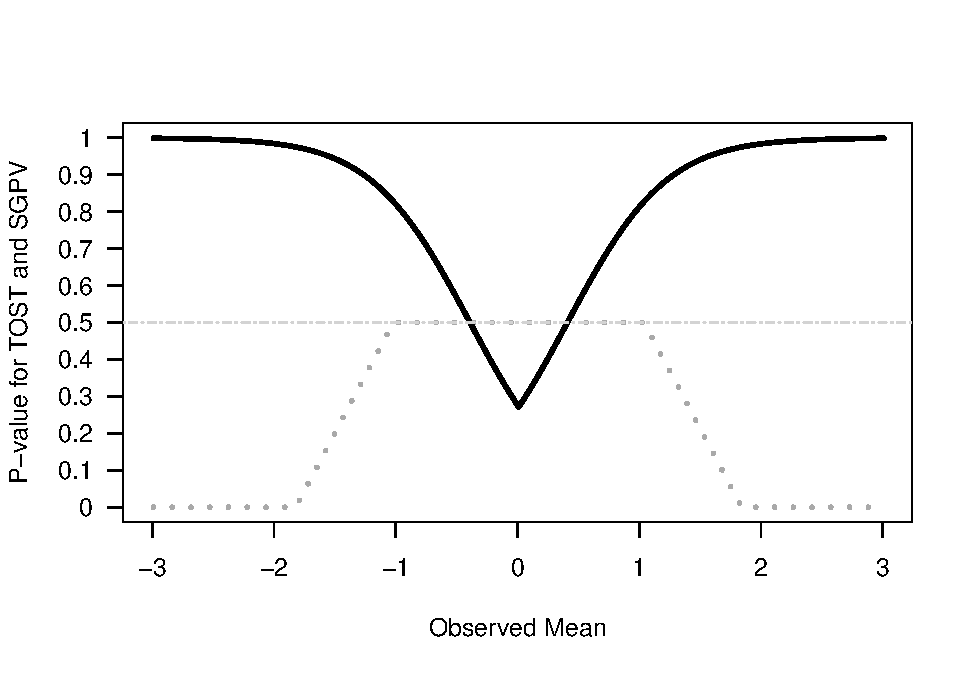
\includegraphics{manuscript_files/figure-latex/TOSTSGPV6-1.pdf}
\caption{\label{fig:TOSTSGPV6}Comparison of \emph{p}-values from TOST (black
line) and SGPV (dotted grey line) across a range of observed sample
means (x-axis). Because the sample size is small (n = 10) and the CI is
more than twice as wide as the equivalence range (set to -0.4 to 0.4),
the SGPV is set to 0.5 (horizontal light grey line) across a range of
observed means.}
\end{figure}

We can examine this situation by calculating the SGPV and performing the
TOST for a situation where sample sizes are small and the equivalence
range is narrow, such that the CI is more than twice as large as the
equivalence range (see Figure \ref{fig:TOSTSGPV6}). When the two
statistics are plotted against each other we can see where they are
unrelated (indicated by straight lines in the curve, see Figure
\ref{fig:TOSTSGPV7}). We see the SGPV is 0.5 for a range of observed
means where the \emph{p}-value from the equivalence test still varies.
It should be noted that in these calculations the \emph{p}-values for
the TOST procedure are \emph{never} smaller than 0.05 (i.e., they do not
get below 0.05 on the y-axis). In other words, we cannot conclude
equivalence based on any of the observed means. This happens because the
TOST \emph{p}-value is smaller than 0.05 only when the 90\% CI falls
completely between the upper and lower equivalence bounds. However, we
are examining a scenario where the 90\% CI is so wide that it never
falls completely within the two equivalence bounds, and thus the
equivalence test is never significant. As Lakens (2017) notes:
\enquote{in small samples (where CIs are wide), a study might have no
statistical power (i.e., the CI will always be so wide that it is
necessarily wider than the equivalence bounds).} None of the
\emph{p}-values based on the TOST procedure are below 0.05, and thus, in
the long run we have 0\% power.

\begin{figure}
\centering
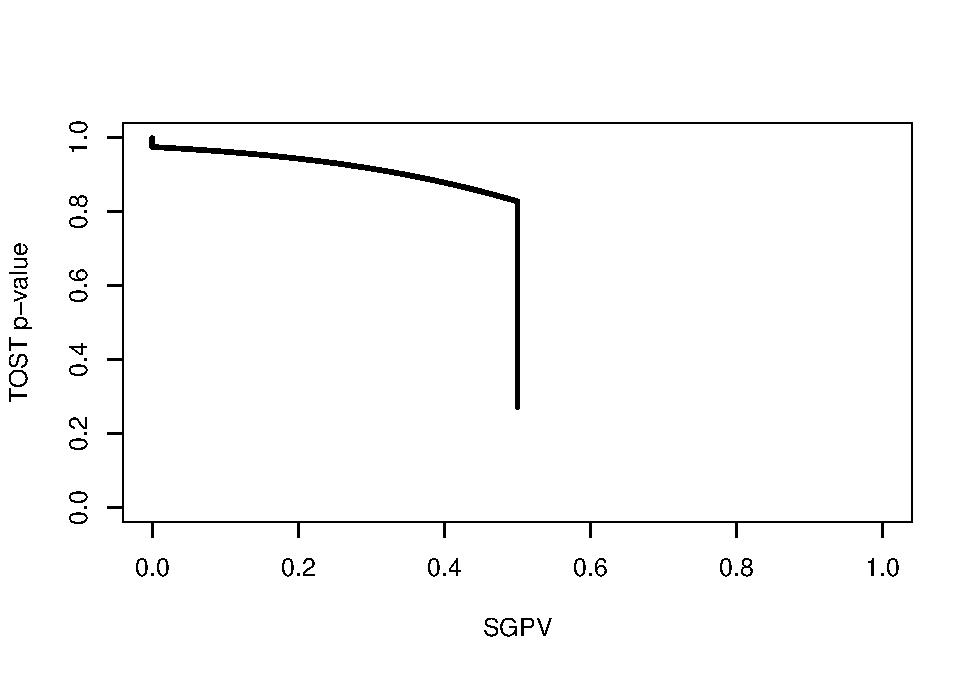
\includegraphics{manuscript_files/figure-latex/TOSTSGPV7-1.pdf}
\caption{\label{fig:TOSTSGPV7}The relationship between \emph{p}-values from
the TOST procedure and the SGPV for the same scenario as in Figure
\ref{fig:TOSTSGPV6}.}
\end{figure}

The \emph{p}-value from the TOST procedure and the SGPV are also
unrelated when the CI is wider than the equivalence range (so the
precision is low) and overlaps with the upper and lower equivalence
bound, but the CI is \emph{not} twice as wide as the equivalence range.
In the example below, we see that the CI is only 1.79 times as wide as
the equivalence bounds, but the CI overlaps with the lower and upper
equivalence bounds (Figure \ref{fig:TOSTSGPV8}). This means the SGPV is
not set to 0.5, but it is constant across a range of observed means.

\begin{figure}
\centering
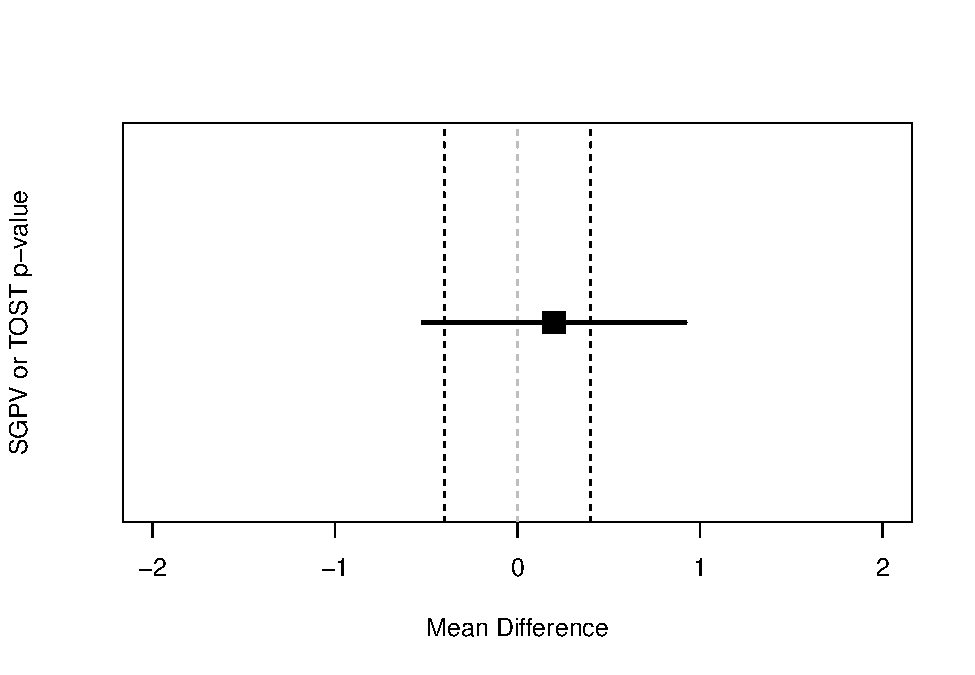
\includegraphics{manuscript_files/figure-latex/TOSTSGPV8-1.pdf}
\caption{\label{fig:TOSTSGPV8}Example of a 95\% CI that overlaps with the
lower and upper equivalence bound (indicated by the vertical dotted
lines).}
\end{figure}

If the observed mean would be somewhat closer to 0, or further away from
0, the SGPV remains constant (the CI width does not change, and it
completely overlaps with the equivalence range) while the \emph{p}-value
for the TOST procedure does vary. We can see this in Figure
\ref{fig:TOSTSGPV9} below. The SGPV is not set to 0.5, but is slightly
higher than 0.5 across a range of means. How high the SGPV will be for a
CI that is not twice as wide as the equivalence range, but overlaps with
the lower and upper equivalence bounds, depends on the width of the CI
and the equivalence range.

\begin{figure}
\centering
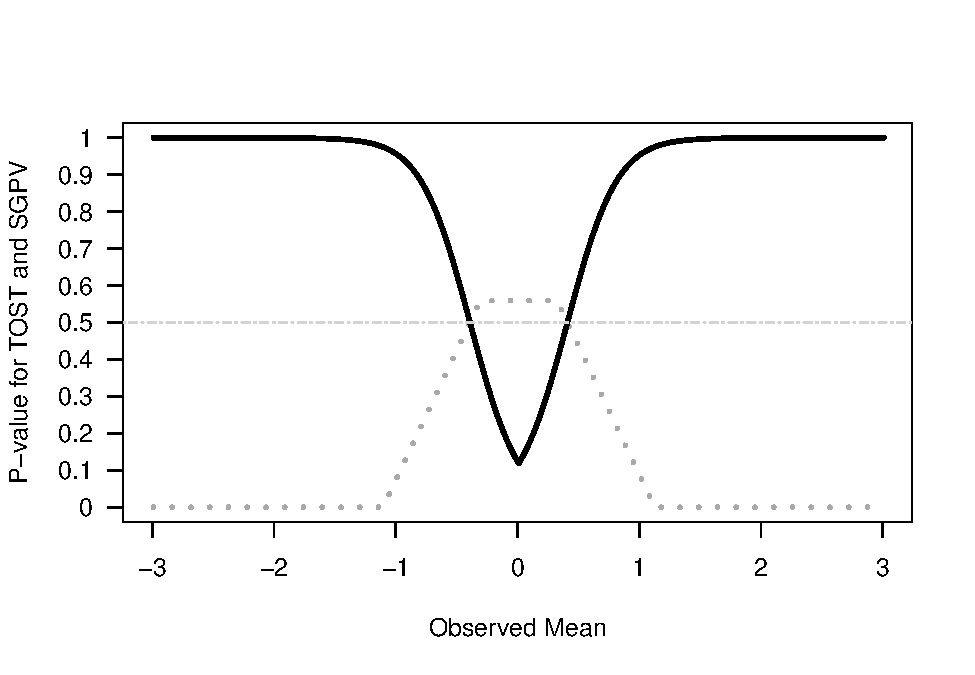
\includegraphics{manuscript_files/figure-latex/TOSTSGPV9-1.pdf}
\caption{\label{fig:TOSTSGPV9}Comparison of \emph{p}-values from TOST (black
line) and SGPV (dotted grey line) across a range of observed sample
means (x-axis). The sample size is small (n = 10), but because the sd is
half as big as in Figure \ref{fig:TOSTSGPV7} (1 instead of 2) the CI is
less than twice as wide as the equivalence range (set to -0.4 to 0.4).
The SGPV is not set to 0.5 (horizontal light grey line) but reaches a
maximum slightly above 0.5 across a range of observed means.}
\end{figure}

If we once more plot the two statistics against each other to see where
they are unrelated (indicated by straight lines in the curve), we see
the SGPV is 0.56 for a range of observed means where the \emph{p}-value
from the equivalence test still varies (Figure \ref{fig:TOSTSGPV10}).

\begin{figure}
\centering
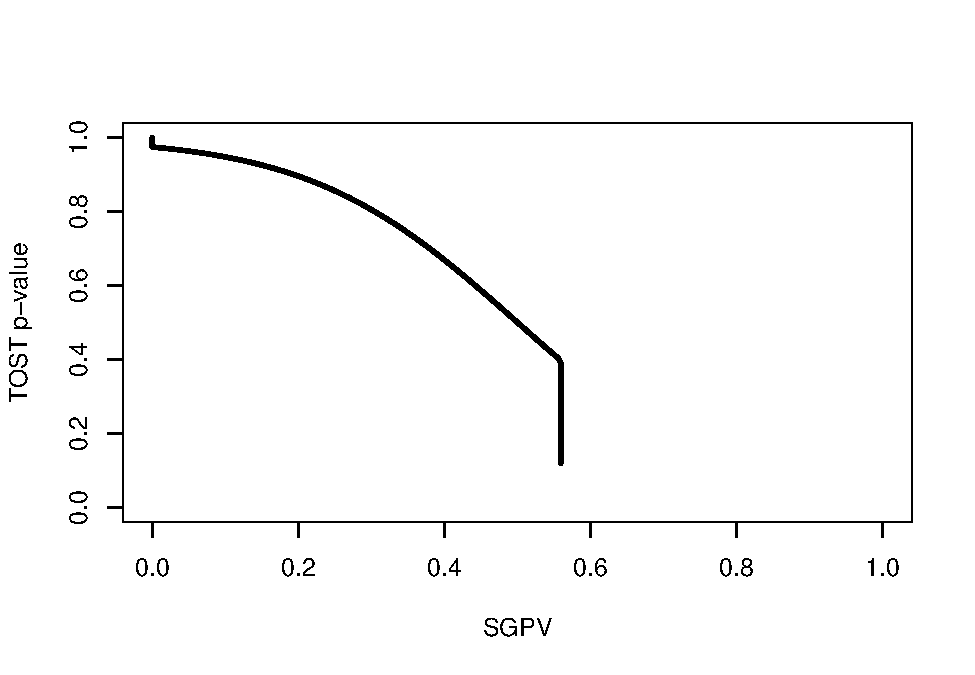
\includegraphics{manuscript_files/figure-latex/TOSTSGPV10-1.pdf}
\caption{\label{fig:TOSTSGPV10}The relationship between \emph{p}-values from
the TOST procedure and the SGPV for the same scenario as in Figure
\ref{fig:TOSTSGPV9}.}
\end{figure}

To conclude this section, there are three situations where the
\emph{p}-value from the TOST procedure is unrelated to the SGPV. In all
these situations the \emph{p}-value for the equivalence test
differentiates tests with different means, but the SGPV does not.
Therefore, as a purely continuous descriptive statistic, the SGPV is
more limited than the \emph{p}-value from the TOST procedure.

\subsection{The relation between equivalence tests and SGPV when
confidence intervals are not
symmetrical}\label{the-relation-between-equivalence-tests-and-sgpv-when-confidence-intervals-are-not-symmetrical}

So far we have only looked at the relation between equivalence tests and
the SGPV when confidence intervals are symmetric (e.g., for confidence
intervals around mean differences). For correlations, which are bound
between -1 and 1, confidence intervals are only symmetric for a
correlation of exactly 0. The confidence interval becomes increasingly
asymmetric as the observed correlation nears -1 or 1. For example, with
ten observations, an observed correlation of 0 has a symmetric 95\%
confidence interval ranging from -0.630 to 0.630, while and observed
correlation of 0.7 has an asymmetric 95\% confidence interval ranging
from 0.126 to 0.993.

The effect of asymmetric confidence intervals is most noticeable at
smaller sample sizes. In Figure \ref{fig:TOSTSGPV11} we plot the
\emph{p}-values from equivalence tests and the SGPV (again plotted as
1-SGPV for ease of comparison) for correlations. The sample size is 30
pairs of observations, and the lower and upper equivalence bounds are
set to -0.45 and 0.45, with an alpha of 0.05. As the observed
correlation in the sample moves from -1 to 0 the \emph{p}-value from the
equivalence test becomes smaller, as does 1-SGPV. The pattern is quite
similar to that in Figure \ref{fig:TOSTSGPV2}. The \emph{p}-value for
the TOST procedure and 1-SGPV are still identical when \emph{p}-values
are 0.975 and 0.025 (indicated by the upper and lower horizontal dotted
lines). There are two important differences, however. First of all, the
SGPV is no longer a straight line, but a curve, due to the asymmetry in
the 95\% CI. Second, and most importantly, the \emph{p}-value for the
equivalence test and the SGPV do no longer overlap at \emph{p} = 0.5.

\begin{figure}
\centering
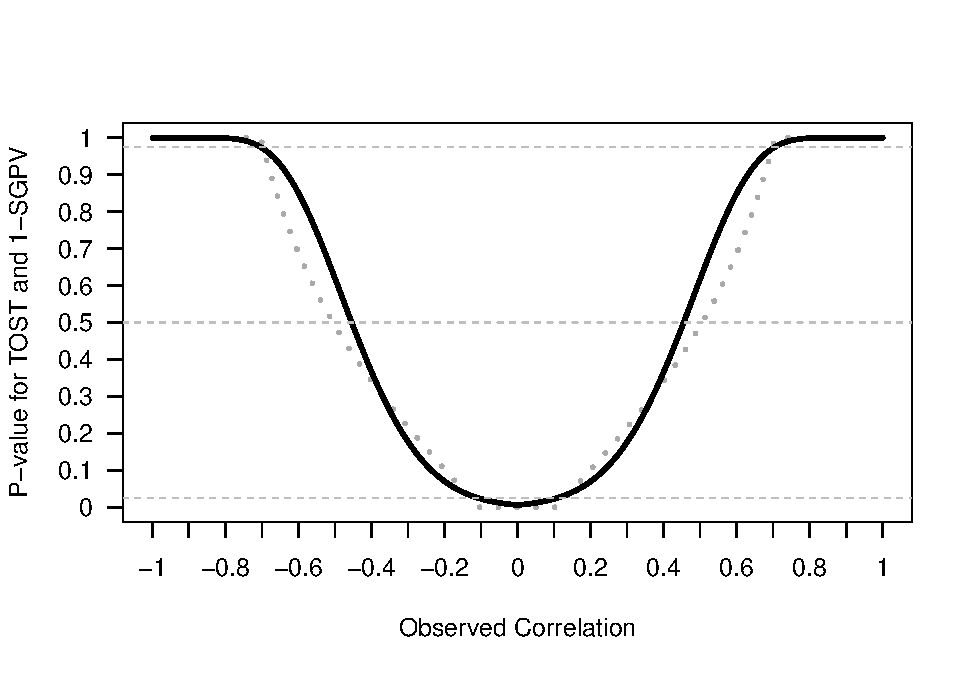
\includegraphics{manuscript_files/figure-latex/TOSTSGPV11-1.pdf}
\caption{\label{fig:TOSTSGPV11}Comparison of \emph{p}-values from TOST
(black line) and 1-SGPV (dotted grey curve) across a range of observed
sample correlations (x-axis) tested against equivalence bounds of r =
-0.45 and r = 0.45 with n = 30 and an alpha of 0.05.}
\end{figure}

The reason that the equivalence test and SGPV no longer overlap is also
because of asymmetric confidence intervals. If the observed correlation
falls exactly on the equivalence bound the \emph{p}-value for the
equivalence test indicates that the probability of observing the
observed or more extreme data, assuming the equivalence bound is the
true effect size, is 50\%. In other words, if the true effect size is
the same as the equivalence bound, it is equally likely to find an
effect more extreme than the equivalence bound, as it is to observe an
effect that is less extreme than the equivalence bound. However, as can
be seen in Figure \ref{fig:TOSTSGPV12}, the two second generation
\emph{p}-values associated with the observed correlations at r = -0.45
and r = 0.45 are larger than 50\%. Because the confidence intervals are
asymmetric around the observed effect size of 0.45 (ranging from 0.11 to
0.70) according to Blume et al. (2018) 58.11\% of the data-supported
hypotheses are null hypotheses, and therefore 58.10\% of the
data-supported hypotheses are compatible with the null premise.

\begin{figure}
\centering
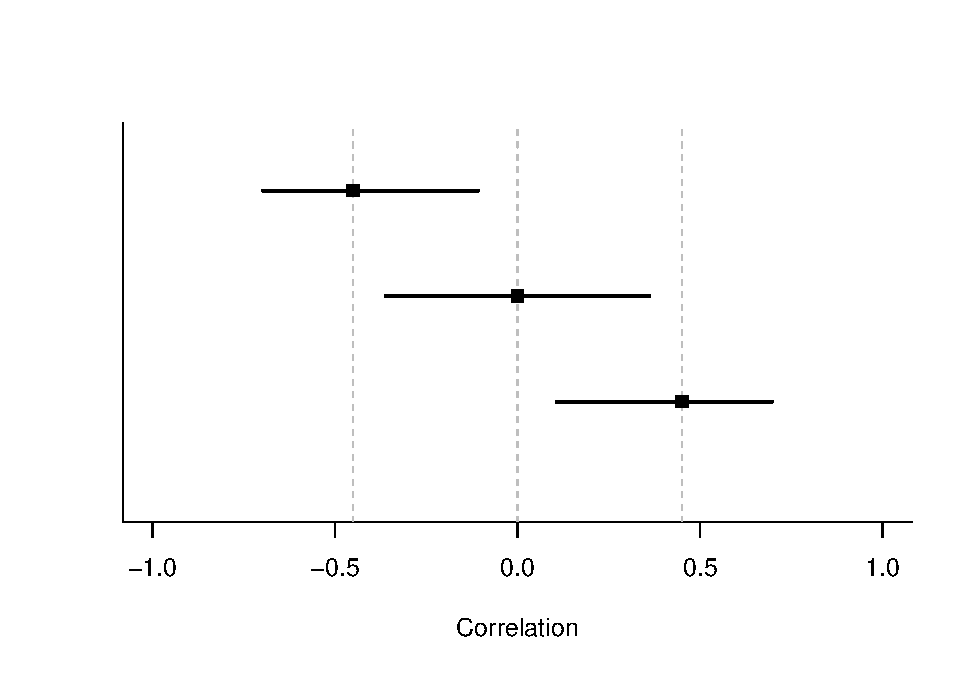
\includegraphics{manuscript_files/figure-latex/TOSTSGPV12-1.pdf}
\caption{\label{fig:TOSTSGPV12}Three 95\% confidence intervals for observed
effect sizes of r = -0.45, r = 0, and r = 0.45 for n = 30. Only the
confidence interval for r = 0 is symmetric.}
\end{figure}

This example illustrates the difference between a proportion and a
probability. There is always a 50\% probability of observing a
correlation smaller or larger than the true correlation, but the SGPV
for this situation depends on how far away the observed correlation is
from 0. The further away from 0, the larger the SGPV when the observed
mean falls on the equivalence bound. The SGPV is the proportion of
values in a 95\% confidence interval that overlap with the equivalence
range, but not the probability that these values will be observed. In
the most extreme case (i.e., a sample size of 4, and equivalence bounds
set to r = -0.99 and 0.99, with an observed correlation of 0.99) 58.10\%
of the confidence interval overlaps with the equivalence range, even
though in the long run only 50\% of the correlations observed in the
future will fall in this range. It should be noted that in larger sample
sizes the SGPV is closer to 0.5 whenever the observed correlation falls
on the equivalence bound, but this extreme example nevertheless clearly
illustrates the difference between question the SGPV answers, and the
question a \emph{p}-value answers. The conclusion of this section on
asymmetric confidence intervals is that a SGPV of 1 or 0 can still be
interpreted as a \emph{p} \textless{} 0.025 or \emph{p} \textgreater{}
0.975 in an equivalence test, since the SGPV and \emph{p}-value for the
TOST procedure are always directly related at these values. Although
Blume et al. (2018) state that \enquote{the degree of overlap conveys
how compatible the data are with the null premise} this definition of
what the SGPV provides does not hold for asymmetric confidence
intervals. Although a SGPV of 1 or 0 can be directly interpreted, a SGPV
between 0 and 1 is not interpretable as \enquote{compatibility with the
null hypothesis}. Indeed, Blume and colleagues write in the supplemental
material that \enquote{The magnitude of an inconclusive
second-generation \emph{p}-value can vary slightly when the effect size
scale is transformed. However definitive findings, i.e.~a \emph{p}-value
of 0 or 1 are \emph{not} affected by the scale changes.}

\subsection{What are the Relative Strengths and Weaknesses of
Equivalence Testing and the
SGPV?}\label{what-are-the-relative-strengths-and-weaknesses-of-equivalence-testing-and-the-sgpv}

When introducing a new statistical method, it is important to compare it
to existing approaches and specify its relative strengths and
weaknesses. First of all, the SGPV is a descriptive statistic (unlike
the \emph{p}-value that is calculated for an equivalence test, which is
an inferential statistic) that provides the proportion of overlap of the
confidence interval and the equivalence range. Even though a SGPV of 1
or 0 has a clear interpretation (we can reject effects outside or inside
the equivalence range), intermediate values are not as easy to interpret
(especially for effects that have asymmetric confidence intervals). In
one sense, they are what they are (the proportion of overlap), but it
can be unclear what this number tells us about the data we have
collected. This is not too problematic, since the main use of the SGPV
(e.g., in all examples provided by Blume and colleagues) seems to be to
examine whether the SGPV is 0, 1, or inconclusive. This interpretation
of a SGPV as allowing researchers to reject the null, reject the
presence of a meaningful effect, or remaining inconclusive is very
similar to the Neyman-Pearson interpretation of combining a
null-hypothesis test and an equivalence test (Lakens et al., 2018). The
difference is that where a SGPV of 1 can be interpreted as \emph{p}
\textless{} .025, equivalence tests provide exact \emph{p}-values, and
they continue to differentiate between for example \emph{p} = 0.048 and
\emph{p} = 0.002. Whether this is desirable depends on the perspective
that is used. From a Neyman-Pearson perspective on statistical
inferences the main conclusion is based on whether or not
\(p < \alpha\), and thus an equivalence test and SGPV can be performed
by simply checking whether the confidence interval falls within the
equivalence range, just as a null-hypothesis test can be performed by
checking whether the confidence interval contains zero or not. At the
same time, it is recommended to report exact \emph{p}-values (American
Psychological Association, 2010), and exact \emph{p}-values might
provide information of interest to readers about how precisely how
surprising the data is under the null model. Equivalence tests combined
with null-hypothesis significance tests also allow researchers to
conclude an effect is significant \emph{and} equivalent (i.e.,
statistically different from zero, but also too small to be considered
meaningful). Thus, the SGPV is used to classify results into one of
three possible categories (with the data falling inside or outside the
equivalence range, or being inconclusive), while equivalence tests
combined with null-hypothesis tests classify results into four possible
categories.

An important issue when calculating the SGPV is its reliance on the
\enquote{small sample correction}, where the SGPV is set to 0.5 whenever
the ratio of the confidence interval width to the equivalence range
exceeds 2:1 and the CI overlaps with the upper and lower bounds. This
exception to the normal calculation of the SGPV is introduced to prevent
misleading values. Without this correction it is possible that a
confidence interval is extremely wide, and an equivalence range is
extremely narrow, which without the correction would lead to a very low
value for the SGPV. Blume et al. (2018) suggest that under such a
scenario \enquote{the data favor alternative hypotheses}, even when a
better interpretation would be that there is not enough data to
accurately estimate the true effect compared to the width of the
equivalence range. Although it is necessary to set the SGPV to 0.5
whenever the ratio of the confidence interval width to the equivalence
range exceeds 2:1, it leads to a range of situations where the SGPV is
set to 0.5, while the \emph{p}-value from the TOST procedure continues
to differentiate (see for example Figure \ref{fig:TOSTSGPV6}). An
important benefit of equivalence tests is that is does not need such a
correction to prevent misleading results.

\begin{figure}
\centering
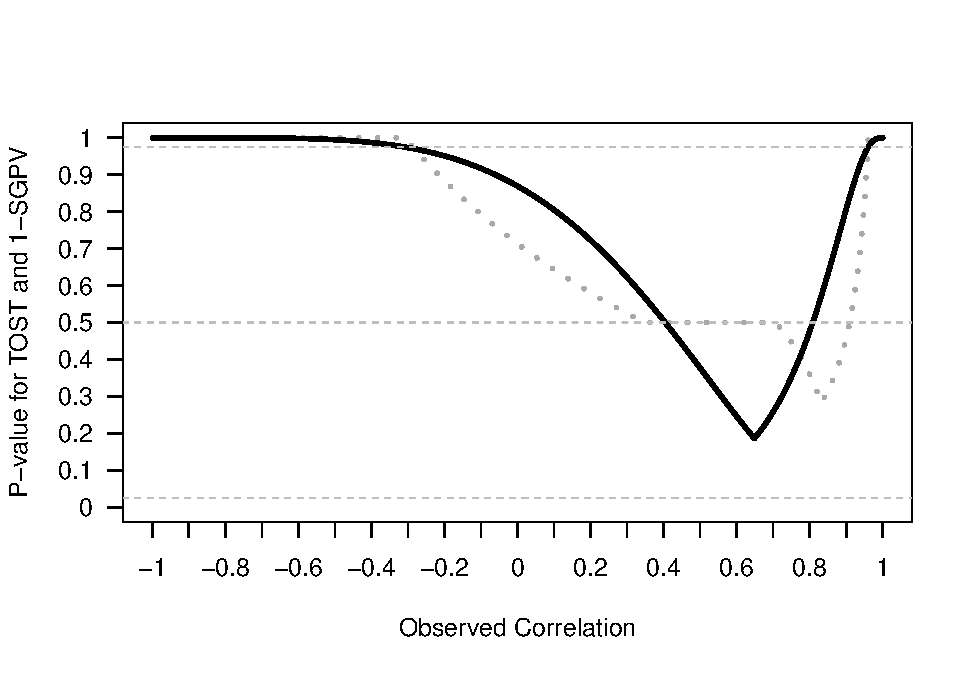
\includegraphics{manuscript_files/figure-latex/TOSTSGPV13-1.pdf}
\caption{\label{fig:TOSTSGPV13}Comparison of \emph{p}-values from TOST
(black line) and 1-SGPV (dotted grey curve) across a range of observed
sample correlations (x-axis) tested against equivalence bounds of r =
0.4 and r = 0.8 with n = 10 and an alpha of 0.05.}
\end{figure}

As a more extreme example of the peculiar behavior of the \enquote{small
sample correction} as currently implemented in the calculation of the
SGPV see Figure \ref{fig:TOSTSGPV13} below. In this figure observed
correlations (from a sample size of 10) from -1 to 1 are tested against
an equivalence range from r = 0.4 to r = 0.8. We can see the SGPV has a
peculiar shape because it is set to 0.5 for certain observed
correlations, even though there is no risk of a \enquote{misleading}
SGPV in this range. This example suggests that the current
implementation of the \enquote{small sample correction} could be
improved. If, on the other hand, the SGPV is mainly meant to be
interpreted when it is 0 or 1, it might be preferable to simply never
apply the \enquote{small sample correction}.

Blume et al. (2018) argue that the SGPV has improved error control, in
that the conclusion that the 95\% confidence interval lies completely
outside the equivalence range around zero will necessarily occur less
frequently than a Type I error in a null-hypothesis test (where the 95\%
confidence interval only needs to not overlap with zero). However, the
SGPV has a \emph{lower} error rate than a null-hypothesis test, not a
\emph{more accurate} error rate. In a Neyman-Pearson perspective (which
forms the basis of equivalence tests) the goal is not to end up with an
error rate that is as low as possible (to achieve that, one simply
adjusts the alpha level), but with a decision procedure that, when
applied, yields a desired error rate with high accuracy. We show here
that the SGPV and equivalence tests are directly related, and so are
their error rates. The TOST procedure uses a 90\% confidence interval
because it is based on two \emph{one-sided} tests, and thus the
confidence interval is 1-2\(\times\)\(\alpha\), and because both tests
need to be significant to conclude equivalence, no adjustment for
multiple comparisons is needed. The TOST procedure always has higher
power to declare equivalence than the SGPV, which relies on a 95\%
confidence interval (but note that there is no reason to always set the
alpha level to 0.05).

Blume et al. (2018) claim that \enquote{Adjustments for multiple
comparisons are obviated} (p.~15) and that \enquote{second-generation
\emph{p}-values provide a proper scientific adjustment for multiple
comparisons}. However, this is not correct. With a sufficient number of
looks error rates can rise above the nominal alpha level (both when
compared to equivalence and minimal effect tests, but even when compared
to a null-hypothesis test). When directly comparing equivalence tests
and the SGPV, multiple comparisons inflate the probability that one
erronously concludes there is \emph{no} effect, where there \emph{is} a
true effect size that equals the equivalence bound, just as quickly for
the SGPV as for equivalence tests, because they are directly related. To
conclude, the idea that the SGPV improves error rates does not hold up
under closer scrutiny, and the recommendation to ignore adjustments for
multiple comparisons has the potential to increase false positives in
the literature. Equivalence tests provide an easier and more formal way
to control both Type I error rates (by setting the alpha level) and the
Type II error rate (by performing an a-priori power analysis).

\section{Conclusion}\label{conclusion}

We believe that our explanation of the similarities between the TOST
procedure and the SGPV provides context to interpret the contribution of
second generation \emph{p}-values to the statistical toolbox. The
novelty of the SGPV lies in its use as a descriptive statistic, but this
use can be limited when confidence intervals are asymmetrical or wider
than the equivalence range. There are strong similarities with
\emph{p}-values from the TOST procedure, and in all situations where the
statistics yield different results, the behavior of the \emph{p}-value
from the TOST procedure is more consistent and easier to interpret. We
hope this overview of the relationship between the SGPV and equivalence
tests will help researchers to make an informed decision about which
statistical approach provides the best answer to their question. Our
comparisons show that when proposing alternatives to null-hypothesis
tests, it is important to compare new proposals to already existing
procedures. We believe equivalence tests achieve the goals of the second
generation \emph{p}-value while allowing users to more easily control
error rates, and while yielding more consistent statistical outcomes.

\newpage

\section{References}\label{references}

\setlength{\parindent}{-0.5in} \setlength{\leftskip}{0.5in}

\hypertarget{refs}{}
\hypertarget{ref-american_psychological_association_publication_2010}{}
American Psychological Association (Ed.). (2010). \emph{Publication
manual of the American Psychological Association} (6th ed.). Washington,
DC: American Psychological Association.

\hypertarget{ref-blume_second-generation_2018}{}
Blume, J. D., D'Agostino McGowan, L., Dupont, W. D., \& Greevy, R. A.
(2018). Second-generation p-values: Improved rigor, reproducibility, \&
transparency in statistical analyses. \emph{PLOS ONE}, \emph{13}(3),
e0188299.
doi:\href{https://doi.org/10.1371/journal.pone.0188299}{10.1371/journal.pone.0188299}

\hypertarget{ref-hauck_new_1984}{}
Hauck, D. W. W., \& Anderson, S. (1984). A new statistical procedure for
testing equivalence in two-group comparative bioavailability trials.
\emph{Journal of Pharmacokinetics and Biopharmaceutics}, \emph{12}(1),
83--91.
doi:\href{https://doi.org/10.1007/BF01063612}{10.1007/BF01063612}

\hypertarget{ref-kruschke_rejecting_2018}{}
Kruschke, J. K. (2018). Rejecting or Accepting Parameter Values in
Bayesian Estimation. \emph{Advances in Methods and Practices in
Psychological Science}, 2515245918771304.
doi:\href{https://doi.org/10.1177/2515245918771304}{10.1177/2515245918771304}

\hypertarget{ref-lakens_equivalence_2017}{}
Lakens, D. (2017). Equivalence Tests: A Practical Primer for t Tests,
Correlations, and Meta-Analyses. \emph{Social Psychological and
Personality Science}, \emph{8}(4), 355--362.
doi:\href{https://doi.org/10.1177/1948550617697177}{10.1177/1948550617697177}

\hypertarget{ref-lakens_equivalence_2018}{}
Lakens, D., Scheel, A. M., \& Isager, P. M. (2018). Equivalence Testing
for Psychological Research: A Tutorial. \emph{Advances in Methods and
Practices in Psychological Science}, 2515245918770963.
doi:\href{https://doi.org/10.1177/2515245918770963}{10.1177/2515245918770963}

\hypertarget{ref-meyners_equivalence_2012}{}
Meyners, M. (2012). Equivalence tests review. \emph{Food Quality and
Preference}, \emph{26}(2), 231--245.
doi:\href{https://doi.org/10.1016/j.foodqual.2012.05.003}{10.1016/j.foodqual.2012.05.003}

\hypertarget{ref-murphy_statistical_2014}{}
Murphy, K. R., Myors, B., \& Wolach, A. H. (2014). \emph{Statistical
power analysis: A simple and general model for traditional and modern
hypothesis tests} (Fourth edition.). New York: Routledge, Taylor \&
Francis Group.

\hypertarget{ref-quertemont_how_2011}{}
Quertemont, E. (2011). How to Statistically Show the Absence of an
Effect. \emph{Psychologica Belgica}, \emph{51}(2), 109--127.
doi:\href{https://doi.org/10.5334/pb-51-2-109}{10.5334/pb-51-2-109}

\hypertarget{ref-rogers_using_1993}{}
Rogers, J. L., Howard, K. I., \& Vessey, J. T. (1993). Using
significance tests to evaluate equivalence between two experimental
groups. \emph{Psychological Bulletin}, \emph{113}(3), 553--565.
doi:\href{https://doi.org/http://dx.doi.org/10.1037/0033-2909.113.3.553}{http://dx.doi.org/10.1037/0033-2909.113.3.553}

\hypertarget{ref-schuirmann_comparison_1987}{}
Schuirmann, D. J. (1987). A comparison of the two one-sided tests
procedure and the power approach for assessing the equivalence of
average bioavailability. \emph{Journal of Pharmacokinetics and
Biopharmaceutics}, \emph{15}(6), 657--680.

\hypertarget{ref-serlin_rationality_1985}{}
Serlin, R. C., \& Lapsley, D. K. (1985). Rationality in psychological
research: The good-enough principle.

\hypertarget{ref-spiegelhalter_bayesian_1994}{}
Spiegelhalter, D. J., Freedman, L. S., \& Parmar, M. K. (1994). Bayesian
approaches to randomized trials. \emph{Journal of the Royal Statistical
Society. Series A (Statistics in Society)}, 357--416.
doi:\href{https://doi.org/10.2307/2983527}{10.2307/2983527}

\hypertarget{ref-wellek_testing_2010}{}
Wellek, S. (2010). \emph{Testing statistical hypotheses of equivalence
and noninferiority} (2nd ed.). Boca Raton: CRC Press.

\hypertarget{ref-westlake_use_1972}{}
Westlake, W. J. (1972). Use of Confidence Intervals in Analysis of
Comparative Bioavailability Trials. \emph{Journal of Pharmaceutical
Sciences}, \emph{61}(8), 1340--1341.
doi:\href{https://doi.org/10.1002/JPS.2600610845}{10.1002/JPS.2600610845}






\end{document}
